%!TEX root = ../thesis.tex

\chapter{Results}
\textit{Parts of this section incorporate text from published work [The central complex of the larval fruit fly brain] (Lungu et al., 2025)}

\section{Strategy for identifying CX neuropils in the larval brain}

    I used an iterative strategy in finding putative larval central complex neurons. For this, I pattern matched individual cells based on adult CX neurons lineages, morphology, relative location and connectivity. %describe the steps of the process at a bit more length 
    %We adopted a search strategy guided by circuit features of the adult brain CX neuropils.
    Since the adult brain presents fused hemispheres at the midline whereas the larva has not, we placed more emphasis of searching for circuit motifs rather than anatomical similarity, since the larval brain has a brain commisure, while preserving the relative spatial location of a CX neuropil as a constraint.

    These included:
    \begin{enumerate}
    \item Integration of sensory inputs: we searched for synaptic pathways corresponding to the adult's for integrating visual inputs into the PB and EB \citep{hulse2021connectome}, and gustatory inputs into the FB.
    \item Association between centers for memory and spatial navigation: we looked for the characteristic link between the MB, the center for associative memory, and CX neuropils, which includes synapses from MBONs (MB output neurons) to the FB, EB and NO in the adult fly.
    \item Recurrent intra-CX connectivity, such as with columnar neurons relating the PB with the FB and EB, or with the NO.
    \end{enumerate}
    
    \subsection{Identifying larval neuronal lineages that contribute to the larval CX}
    The \textit{Drosophila melanogaster} central brain consists of stereotyped neural lineages, developmental-structural units of macrocircuitry formed by the sibling neurons of single progenitor cells, the neuroblasts \citep{Spindler2010Lineages}, a subset of which structures the CX \citep{Pereanu2011LineagesCX}.
    Starting with the currently identified set of quiescent, embryonic-born neurons present in the larval brain that develop into to the adult CX during metamorphosis~\citep{andrade2019developmentally}
    we identified larval brain neurons satisfying imposed connectivity rules as per known circuit patterns across the adult CX neuropils \citep{wolff2015neuroarchitecture, wolff2018neuroarchitecture, franconville2018building, hulse2021connectome}.

    We broadened the search beyond these lineages based on the expectation that some larval neurons may have been recruited to CX structures but would later take another identity in the adult, as is known for larval MB neurons \citep{truman2023metamorphosis}, on the basis of matching synaptic connectivity patterns as observed in the adult; for example, for EB Ring neurons we looked for neurons with recurrent axo-axonic synapses with each other and with Wedge neurons, where their axon is located at the most anterior end of the brain neuropil, at an intermediate dorso-ventral position just anterior to the MB medial lobe.
    %MY PART 
    %Lineages
    We expected to find neurons originating from DM1, DM2, DM3, DM4, DM5 and DM6 hemilineages as these are core lineages contributing to all neuropils(Table \ref{adultlineages}), with the second priority being neuropil specific lineages(e.g. EBa1(DALv2) for the EB see \ref{adultlineages}). 12 of the 15 lineages found to contribute CX neurons in the adult also exist in the larva. Of these, we found that 9 of them contribute neurons to the larval central complex (Table \ref{lineagemap}). We therefore used these 9 lineages as a starting point to find our putative CX neuropils in the larva.

        \begin{table}
        \centering
        \begin{tabular}{|c|c|}
        \hline
        Adult lineage & Larval lineage \\
        \hline
        DM1 & DPMm1 \\
        DM2 & DPMpm1 \\
        DM3 & DPMpm2 \\
        DM4 & CM4 \\
        DM5/DM6 & CM1/3 \\
        DL1 & CP23 \\
        EBa1 & DALv2 \\
        LALv1 & BAMv1 \\
        CREa1 & BAmd1 \\
        CREa2 & DALCm12 \\
        SMPad2 & DAMd2/3 \\
        SIPp1 & DPMpl12 \\
        \bottomrule
        \end{tabular}
        \caption[Lineges of the Adult CX that also contribute neurons to the Larval CX]{\textbf{Lineges of the Adult CX that also contribute neurons to the Larval CX} Adult CX lineages are listed in the first column, and their corresponding larval lineages in the second.}
        \label{lineagemap}
        \end{table}

    In addition to the lineages that contribute to the adult CX, there were several neurons from other lineages, which satisfied other criteria (such as connectivity patterns or relative location) and were therefore classified as central complex neurons. These lineages are presented in Table \ref{larvallineages} which containts all the lineages we found to contribute neurons to the larval CX. None of these lineages are exclusive contributors to the larval CX - i.e all of these lineages contribute neurons to other parts of the brain - however, there are a few(about 10) that contribute more than a fifth (20\%) of their neurons to CX neuropils (Figure (\ref{cx_percentage})).


    \begin{table}
    \centering
    \resizebox{\textwidth}{!}{%
    \begin{tabular}{|c|c|c|c|c|c|c|c|c|c|}
    \toprule
    Larval lineages & PB.b & PB.d & FB.b & FB.d & EB.b & EB.d & NO.b & NO.d & Total \\
    \midrule
    BAla12 &  &  &  & 2 & 2 &  &  &  & 4 \\
    BAla34 &  &  & 4 &  &  &  &  & 9 & 13 \\
    BAlp\_ant &  & 2 &  &  & 2 &  &  & 1 & 5 \\
    bamd1 &  &  &  &  &  & 1 &  & 2 & 3 \\
    bamd2\_d &  &  & 1 &  &  &  &  &  & 1 \\
    bamd2\_v &  &  & 3 &  &  &  &  & 4 & 7 \\
    bamv12\_dor & 1 &  &  & 1 &  &  & 2 & 5 & 9 \\
    BAmv12\_dor & 1 &  &  & 1 &  &  & 2 & 5 & 9 \\
    Bamv12\_ven & 1 &  &  & 1 & 2 & 2 &  & 1 & 7 \\
    BLAd-OL & 2 &  &  &  &  &  &  &  & 2 \\
    BLAl &  &  &  & 2 &  &  &  &  & 2 \\
    BLAV12\_ant &  &  &  & 2 &  &  &  &  & 2 \\
    BLP12 &  &  &  &  &  & 2 &  &  & 2 \\
    BLVp2 &  & 2 &  &  &  &  &  &  & 2 \\
    CM13\_lat &  & 2 &  &  & 4 & 2 &  &  & 8 \\
    CM13\_med &  &  &  &  & 2 & 2 &  &  & 4 \\
    CM4-vm &  &  &  & 2 &  &  &  & 4 & 6 \\
    CPa &  &  & 1 &  &  &  &  &  & 1 \\
    CPb &  &  &  &  & 8 & 4 &  &  & 12 \\
    CPe &  &  &  & 2 &  &  &  & 4 & 6 \\
    Dalcl12 &  &  &  &  & 16 & 22 &  &  & 38 \\
    Dalcm12-m &  &  &  &  &  & 4 &  & 2 & 6 \\
    DALcm12-v &  & 2 &  & 2 &  &  & 4 & 1 & 9 \\
    dall1 &  & 2 & 4 &  &  &  &  &  & 6 \\
    Dalv1 & 8 &  &  & 6 &  &  &  &  & 14 \\
    Dalv23 &  &  &  &  & 14 &  &  & 4 & 18 \\
    dplal1-3 &  &  & 2 &  & 3 &  &  &  & 5 \\
    dplc\_post\_med &  & 4 &  & 2 &  &  & 4 &  & 10 \\
    DPLc5 &  & 6 & 1 & 2 &  &  & 3 &  & 12 \\
    DPMl\_ant & 3 & 2 &  &  &  &  &  & 3 & 8 \\
    DPMl12 &  & 3 &  & 2 &  &  & 2 &  & 7 \\
    DPMl34\_post &  &  &  & 1 &  &  & 1 &  & 2 \\
    DPMm1 & 4 &  & 14 & 2 &  &  & 4 &  & 24 \\
    DPMm2 &  & 3 &  & 2 &  & 2 &  &  & 7 \\
    DPMpl12 &  & 5 & 2 & 2 &  &  &  &  & 9 \\
    dpmpl3 &  &  &  &  &  &  &  & 1 & 1 \\
    DPMpm1 &  &  & 4 & 2 &  & 4 &  &  & 10 \\
    DPMpm2 &  &  &  &  &  & 2 & 2 &  & 4 \\
    \bottomrule
    Total & 20 & 33 & 36 & 36 & 53 & 47 & 24 & 46 & 295 \\
    \bottomrule
    \end{tabular}
    }
    \caption[Larval Central Complex Lineages]{\textbf{Larval Central Complex Lineages.} A full list of Larval CX lineages is shown in the first column. If a lineage also contributes to the adult CX, the corresponding adult nomenclature \citep{eckstein2024neurotransmitter} is shown in the second column. Columns 3--6 indicate the number of neurons from each lineage that contribute axons (“.b” for boutons) or dendrites (“.d”) to individual neuropils: PB, FB, EB and NO.}
    \label{larvallineages}
    \end{table}

    % green gradient 
    \definecolor{forest1}{HTML}{EAF2E3} 
    \definecolor{forest2}{HTML}{D7E8C9}
    \definecolor{forest3}{HTML}{B9D89C}
    \definecolor{forest4}{HTML}{93C47D}
    \definecolor{forest5}{HTML}{6AA84F} 

    \begin{table}[h!]
\centering
\begin{tabular}{|l|c|c|c|c|}
\hline
\textbf{Lineage} & \textbf{Left Hemisphere} & \textbf{Right Hemisphere} & \textbf{CX neurons} & \textbf{CX \% of Lineage} \\
\hline
Dalcl12 & 25 & 27 & 38 & \cellcolor{forest5}73.08\% \\
Dalv1 & 11 & 11 & 14 & \cellcolor{forest4}63.64\% \\
dplc\_post\_med & 6 & 10 & 10 & \cellcolor{forest4}62.50\% \\
DPMl12 & 13 & 2 & 7 & \cellcolor{forest3}46.67\% \\
Dalv23 & 18 & 21 & 18 & \cellcolor{forest3}46.15\% \\
DPLc5 & 13 & 14 & 12 & \cellcolor{forest3}44.44\% \\
dplal1-3 & 2 & 12 & 5 & \cellcolor{forest2}35.71\% \\
CPb & 14 & 20 & 12 & \cellcolor{forest2}35.29\% \\
DPMm1 & 38 & 47 & 24 & \cellcolor{forest1}28.24\% \\
dall1 & 9 & 18 & 6 & \cellcolor{forest1}22.22\% \\
\hline
\end{tabular}
\caption[Contribution of lineage to CX]{\textbf{Lineage contribution to CX}  This table illustrates lineages that contribute more that 20\% of their neurons ot the CX. the second and third column show their distribution across the brain hemispheres, whilst tha last column shows the percentage of neurons that contribute(axons, dendrites or both) to CX neuropils}
\label{cx_percentage}
    \end{table}

    \subsection{Connectivity of CX neurons}
    %CONNECTIVITY
    To be able to identify which neurons could contribute to the CX, we investigated their connectivity patterns. Specifically,we summarised where a neuron receives synaptic input (location of its dendrites) and sends output processes (location of its axons).
    %Sensory
    The central complex is known primarily for visual input processing, therefore in the larva we were looked at neurons downstream of photoreceptors. We investigated cells immediately connected to visual projection neurons (vPNs) which are directly connected to photoreceptors. Several of these neurons have been catalogued as Protocerebral Bridge (see section \ref{PB}) or Noduli(see section \ref{NO}) neurons. 
    In additon to visual input, we find that olfactory input is integrated by all the larval CX neuropils indirectly via the Lateral Horn(LH) and the Mushroom Body through convergence neurons(CNs; which integrate learnt valences from the MB and innate valences from the LH \citep{eschbach2021circuits}) or MB output neurons and MB input neurons. This is in line with previous findings about the CX being integrative across multiple sensory modalities \citep{hulse2021connectome}. Since Gepner et al., 2015 demonstrated that Larvae  have to integrate visual and olfactory gradients, with convergence of these sensory systems before decision to act on themwe expected there would be a structure recieving input from these modalities and used information such as lineage membership to figure out if these could be central complex neurons. 

    %Input from other neuropils/lal
    Columnar and horizontal neurons have stereotyped connectivity patterns within the CX, being connected between themselves or with other accessory structures (e.g.LAL). To be able to define these, we categorised them similarly to how they have been categorised in the literature. For naming, we adapted Wolff et al., 2015 nomenclature, and named them on the baisis of the location of input synapses (.d for dendrites) and the location of their output synapses (.b for axonal bouttons). Once the synapses for each neuron was mapped, we categorised them on the basis of their location within the CX neuropils and relative to accesory structures as per Figure \ref{CXclasses}.  As such we devided them into Intrinsic Neurons(those whose inputs and outputs are located within CX neuropils), Local Neurons (cells whose inputs and outputs located within the same neuropil), Input Neurons (those that send only dendrites processes within the CX and output outside of it) and Output Neurons: Cells that send denritic inputs outside of the CX but output onto the CX neuropils. Since the CX of the larva is numerically reduced, we grouped Intrinsic and Local neurons, and named these \textbf{Core CX neurons} for a more concise, cohesive analysis of the CX network. There are 15 pairs of CX core neurons, all of which are presented in Table \ref{CXCoreNeurons}. For a comprehensive understanding of the connectivity patterns of these neurons, they have been written in a nomenclature adapted from Wolff et al., 2015 \citep{wolff2015neuroarchitecture}. We classified neurons using the suffixes ".b" (axon boutons) and ".d" (dendrites) for CX neuropils.
    Hence, a neuron annotated as NO.b projects its axon into the NO, and likewise, a neuron annotated as FB.d places its dendrites in the FB.
    As such, neurons that are both .b and .d for CX neuropils are the CX Core neurons. 



            \begin{figure}
                \centering
                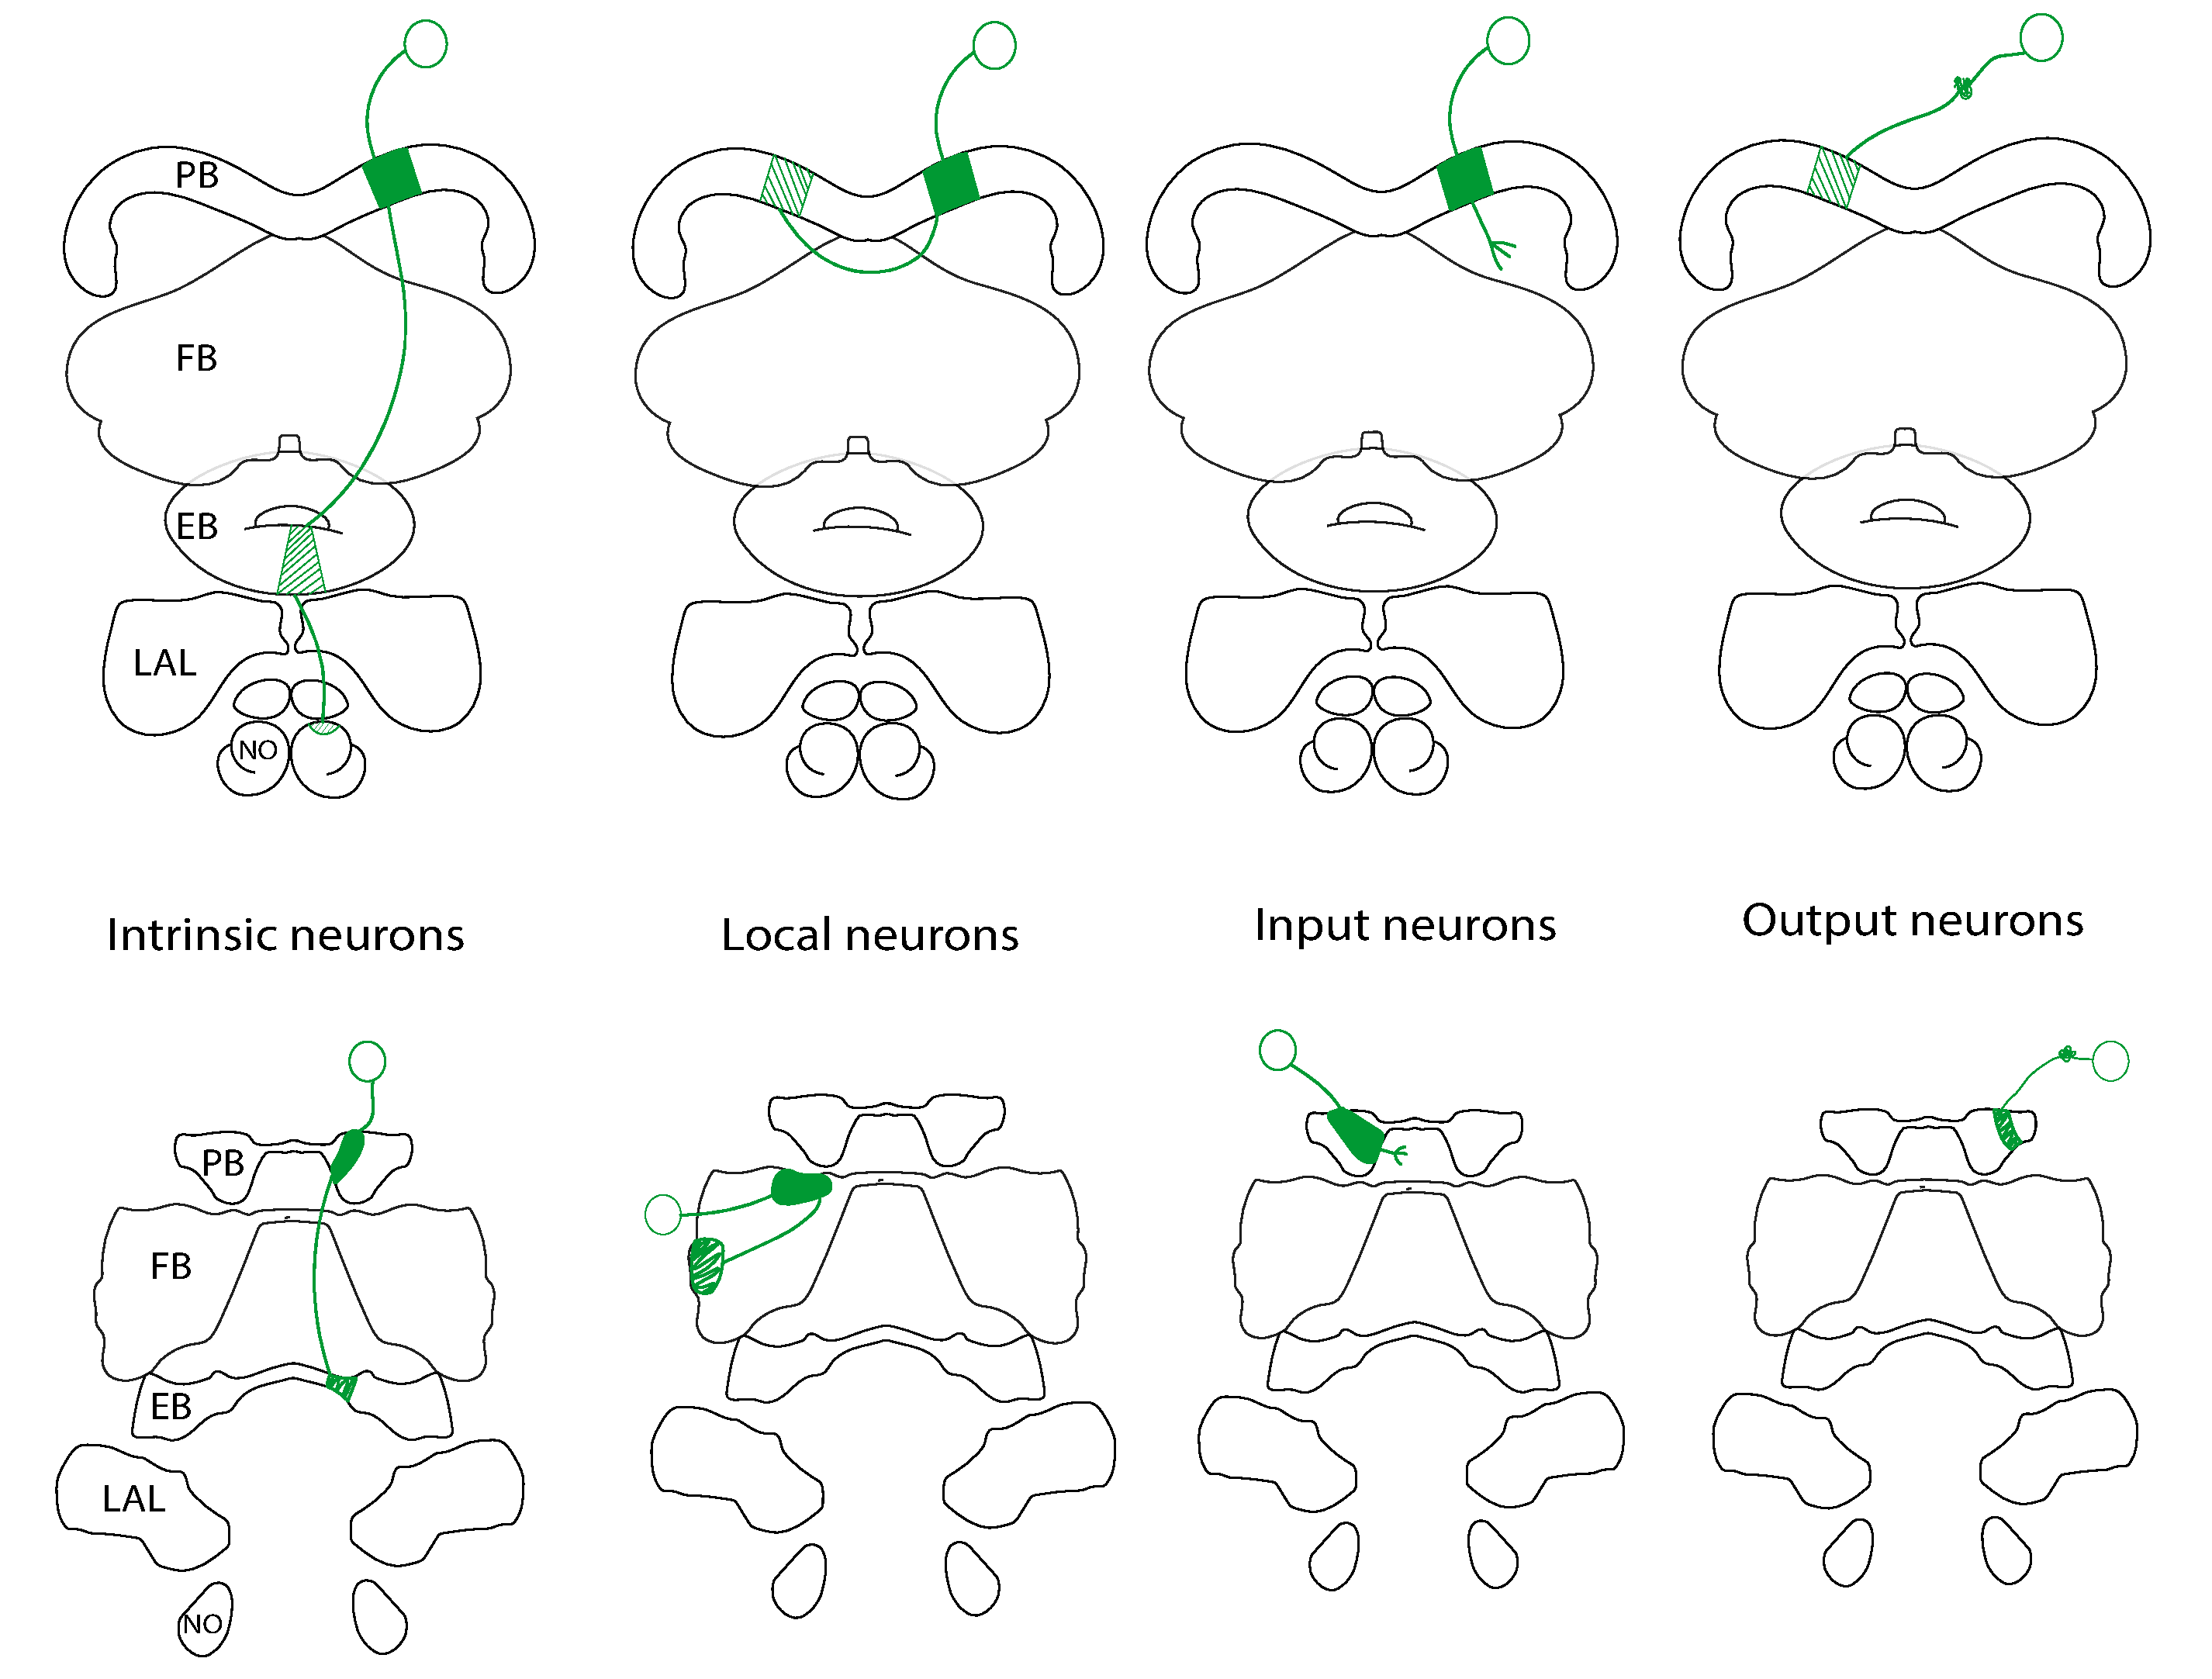
\includegraphics[width=12cm]{Figs/CX/CX_Nomenclature_Neurons.pdf}
                \caption[Central Complex Neuron Classes]{\textbf{Classes of CX neurons} This schematic illustrates neuron classes of the adult CX (upper panel) and the larval CX (lower panel). The PB, FB, EB, NO and LAL are shown in each case to illustrate where a neuron arborizes. Neurons are drawn as a sketch, where the soma is represented by a green circle, the arbors are split into dendritic inputs - filled green boxed - and spiny axonal outputs - hashed scribbled green boxes. Cells are classified as either \textbf{Intrinsic Neurons}:neurons whose inputs and outputs are located within CX neuropils; \textbf{Local Neurons}: cells whose inputs and outputs located within one neuropil; \textbf{Input Neurons}: Neurons that have  dendrites (receive synaptic input) located within the CX but output outside of it; and \textbf{Output Neurons}: Cells that receive inputs outside of the CX but output onto CX neuropils}
                \label{CXclasses}
            \end{figure}

            \begin{table}[h!]
            \centering
            \begin{tabular}{|l|l|}
            \hline
            \textbf{CX Core Neurons} & \textbf{Other Names (CX or MB)} \\
            \hline
            FB.d, NO.b & FB-NO 1, FB.d.1 \\
            FB.d, PB.d, NO.b & FB.d.1, CN-34, MB2ON-119 \\
            FB.d, PB.d, NO.b & FB.d.1, MB2ON-204 \\
            FB.d, NO.b & FB.d.1, MB2ON-201 \\
            EB.d, EB.b, LAL.b & MB2IN-124, MB2ON-79 \\
            EB.d, LAL.d, EB.b & RN4, FBN-19, MB2IN-37, MB2ON-112 \\
            EB.d, LAL.d, EB.b & RN4, FBN-21, MB2IN-42, MB2ON-128 \\
            EB.d, EB.b & RN3, MB2IN-122, MB2ON-71 \\
            EB.d, EB.b & RN1/2a, FBN-20, MB2IN-38, MB2ON-115 \\
            EB.d, EB.b & RN1/2b, FB2IN-10, MB2IN-68, MB2ON-266 \\
            FB.d, FB.b & eDAN-2 \\
            FB.d, FB.b & MB2ON-125 \\
            FB.d, LAL.b & FB.d.2 \\
            PB.d, FB.d & FB.d.2 \\
            PB.d, NO.b & MB2ON-241 \\
            \hline
            \end{tabular}
            \caption[CX Core Neurons]{\textbf{CX Core Neurons} The table illustrates, in the first column, the CX Core neurons in nomenclature adapted from Wolff et al., 2015\citep{wolff2018neuroarchitecture}, depicting the location of the dendrites (.d) axonal butons (.b) in the Central Complex Neuropils. Each neuron is listed alongside their CX neuropil-specific nomenclature, and/or their MB nomenclature}
            \label{CXCoreNeurons}
            \end{table}


    


\section{The Central Complex Adult vs Larva}
    \begin{figure}
        \centering
        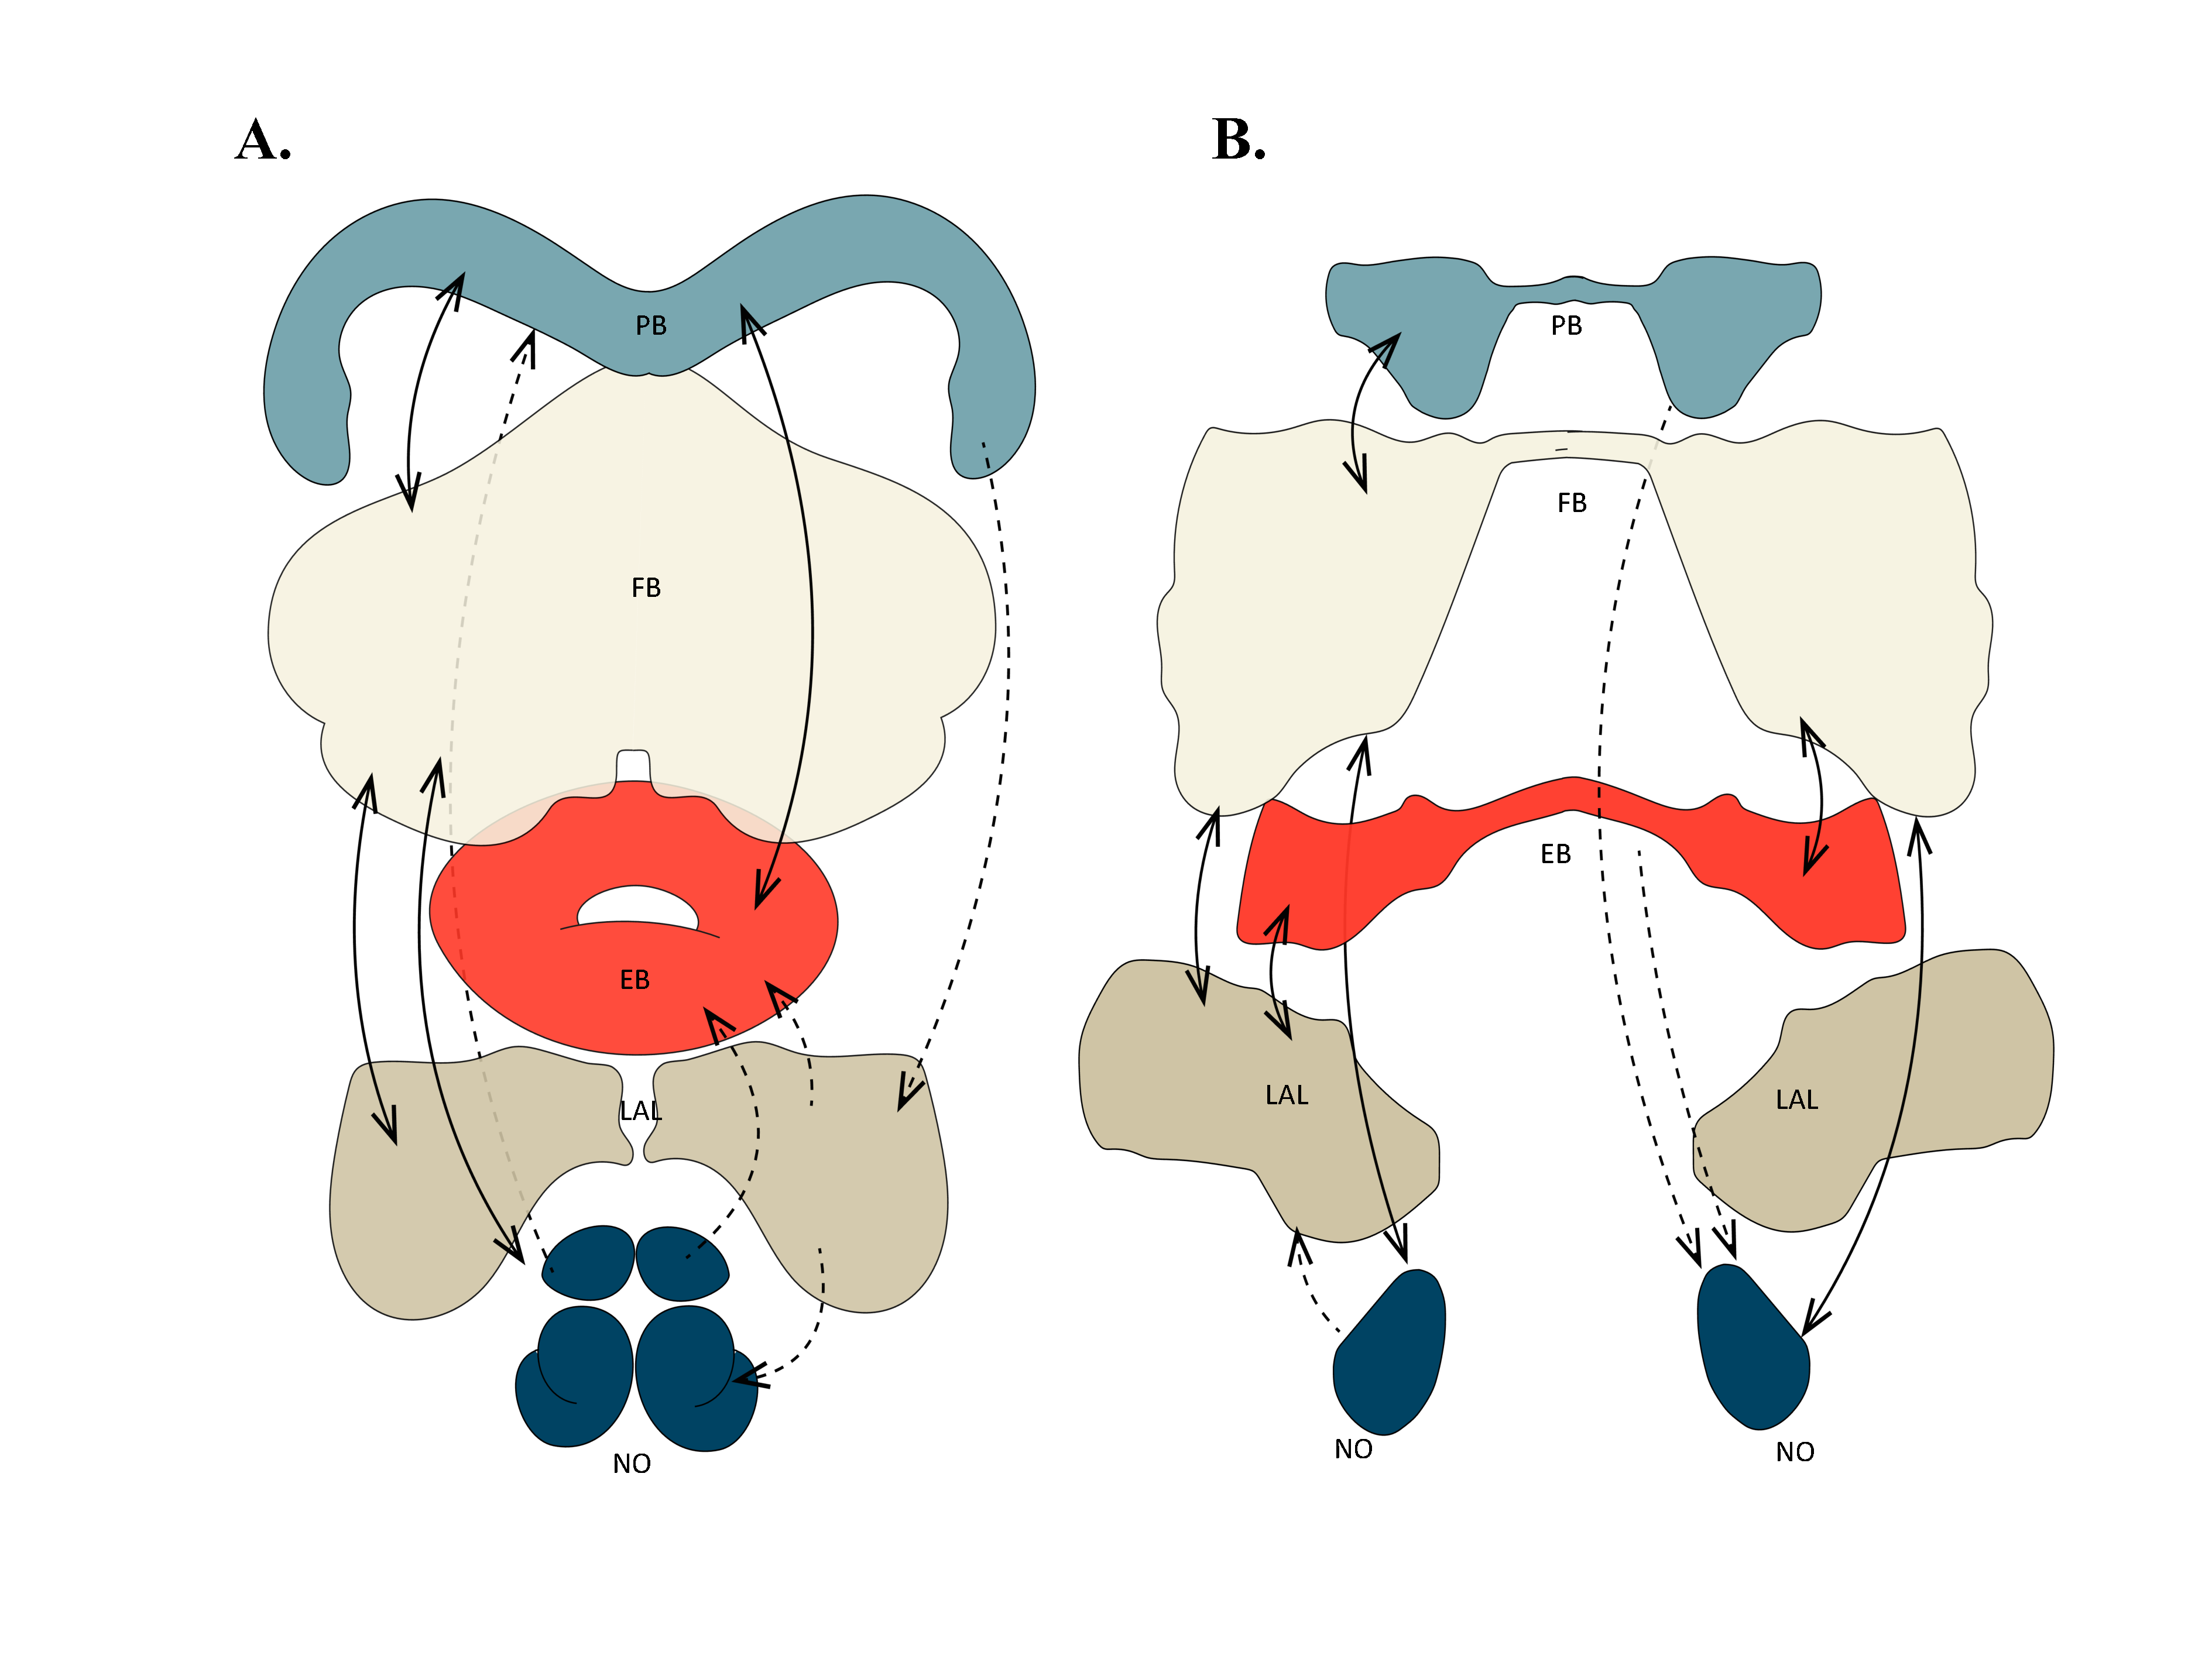
\includegraphics[width=12cm]{/Users/lauralungu/Desktop/Latex/PhD-Thesis/Figs/CX/cxdiagram.pdf}
        \caption[Central Complex Anatomy Larva vs Adult]{Central Complex Anatomy Larva vs Adult}
        \label{cxdiagram}
    \end{figure}

    \subsection{Protocerebral Bridge}
    \label{PB}
    In searching for the larval PB, we expected two sets of neurons: columnar and horizontal. In larva, four central complex lineages contribute columnar neurons, a subset of which position their dendrites at a posterior-dorsal location. We could not find a central complex lineage that would contribute horizontal fibers at a posterior-dorsal location necessary to intersect and synapse onto the dendrites of the PB columnar neurons, but we found a larval lineage (DALv1) whose axons are bilateral and project to the appropriate area, and is developmentally related to another central complex lineage (DALv23). This suggests that neurons from non-central complex lineages may be recruited temporarily during the larval period, in a pattern reported so far for the mushroom body (see Discussion; \citep{truman2023metamorphosis}). 

    Among neurons of the DALv1 lineage, 4 left-right pairs (named HF-PB for "Horizontal Fiber PB") project their axons bilaterally and across the dendrites of the columnar neurons.
    3 of the 4 pairs present an unusual axon configuration: first, they project contralaterally to drop their first output synapses, with the axon then crossing the midline a second time to return back to the same ipsilaterally corresponding location to again drop presynaptic sites .
    This peculiar axon configuration is unique among all neurons of the entire brain of the larva~(\citep{winding2023connectome}) and suggestive of potentially a delay line for comparing left-right sensory inputs.
    The 4th pair first drops presynaptic sites ipsilaterally and then its axon crosses the midline until reaching the corresponding contralateral location to synapse again~(\ref{FigureX}).

    % Relative to the root of their dendritic tree, which is ipsilateral, the first set of output synapses are found contralaterally. Then the axon crosses the midline a second time, returning to the ipsilateral hemisphere to establish more output synapses in a spatially symmetric way to the contralateral set of output synapses.

    The presynaptic outputs of DALv1 neurons are symmetric, in that they contact the same homologous pairs of left-right neurons which are predominantly neurons of the columnar system ~(\ref{FigureX}).
    The axons of these 4 pairs of HF-PB neurons are tiled dorso-ventrally, falling into two bilaterally symmetric groups which we interpret as defining 2 + 2 bilaterally arranged PB compartments, each innervated by 2 pairs of axons. % figure PB compartments

    The dendrites of these 4 pairs of DALv1 neurons (HF-PB) are ipsilateral and dorsal, receiving polysynaptic inputs from vision and olfaction, like in the adult PB~(\citep{hulse2021connectome}). In the larva, we found that these multi-sensory inputs to the horizontal fibers of the PB are mediated by Convergence Neurons (CN-53 and CN-54, among others; \citealp{eschbach2021}) that, as their name indicates, integrate inputs from both Mushroom Body Output Neurons (MBONs) and from the Lateral Horn (LH) such as olfactory and visual PNs \citep{EsbachFushiki2021}). This circuit architecture indicates that sensory inputs arriving to the larval PB will have been modulated or gated by previously established associative memories, with implications for spatial navigation.

    % check for more CNs or other neurons converging onto PB DALv1 dendrites
    %ANSWER: CN35, CN45, CN9 low syn count CN26, CN15
    %as well as from other sensory modalities (Table \ref{sensoryinputs})
    %TODO: describe dendritic and axonic contributions in specific (especially from AL, OL and MB) 
    %2 systems: pattern of input of dendrites of the DALv1 s.
    % MB2ON-175 & 48 & 208 
    % given the PB1-4 compartments, which ones are connected to the MBONs, and the CNs. 175 targets one compartment, 208 targets another.  The pattern is that CNs connect to one compartment of the PB while simultaneously connecting to another CN that connects to the opposite compartment - there could be a gating mechanism. 
    %MB2ON 202 - feedback from the NO to the PB dalv1 


    In the larva, the columnar system consists of neurons from 4 central complex lineages (DPMpm1, DPMpm2, DPMm1 and CM4) that also generate the columnar neurons of the adult (DM1, DM2, DM3 and DM4, correspondingly).
    Larval columnar neurons present small, narrow dendrites circumscribed within the 2 + 2 compartments defined by the axons of the horizontal fibers (DALv1 neurons), with whom they synapse.
    Among the columnar neurons, a subset project their axons directly to the Noduli (NO; %TODOFig), 
    and another subset project directly to the larval Ellipsoid Body (EB;%TODOfig).
    We did not find in the larva columnar neurons whose axons would project to more than one Central Complex neuropil, despite such types being common in the adult \citep{wolff2015neuroarchitecture, wolff2018neuroarchitecture, hulse2021connectome}.
    Beyond the canonical columnar neurons projecting to other Central Complex neuropils, we found some whose axons descend to the SEZ or nerve cord~(%TODOFig).

    % TODO Discussion point: this is different than in the adult. 

    % QUESTION: in the adult, are there columnar neurons that descend to the nerve cord? We have them too in larvae Should mention I them. %ANSWER: see figure 63A Hulse et al. supplement 1 PFL -> MDNs (I have a feeling mdn is smth else in adult)

    %In the \textit{Drosophila} larva Electron Microscopy (EM) volume, we found a putative PB situated at the most medial-posterior side of the brain, that receives high levels of visual input and is made of neurons belonging to lineages DM2 (DPMpm1 in the larva) and 8 columnar neurons(4 pairs) belonging to the lineage DALv1. 
    % also - a dopaminergic pathway formed by large field CIVP neurons that relay IDFP signals to the entire PB

    \subsection{Ellipsoid Body}
    The adult Ellipsoid Body(EB) is a ring-shaped structure situated between the Fan-Shaped Body(FB) and the Mushroom Body horizontal lobes, facing anterodorsally. Its circuit is made up two types of neurons: ring-neurons (derived mainly from the EBAa1/DALv2 and LALv1/BAmv1/2 lineages) that spread their axons across the length of the EB, and reciprocally connected wedge neurons(derived from the DALcl12 lineage) that divide the EB into 16 compartments (aka. wedges)~\citep{omoto2018neuronal}. 

    Its underlying circuit follows the ring attractor architecture (Zhang, 1996) which, as predicted by its anatomy, is shown to yield neural activity in the form of a topological ring in \textit{Drosophila} adult(Seeling \& Jayaraman 2015) with all nodes being connected via inhibitory connections, complemented by local recurrent excitations that maintain activity at each node once they escape inhibition.%(this last sentence is Stanley Heinze).

    The wedge neurons(EPG) form eight wedges around this ring, and project to both hemispheres of the PB, where they connect to two sets of columnar neurons that project back to the EB, forming recurrent loops. These are PEG and PEN neurons. The anatomical offset between EPG and PEN neurons is key to how the fly head direction system translates angular motion into an updated position of the activity bump in the ring attractor. 


    The EB receives visual inhibitory GABAergic inputs, via two parallel pathways for distinct visual information:
    1. Ring neurons that deconstruct the visual environment of the fly; 2. tangential neurons that take in information about body rotations and transnational velocity. The latter receive input in the LAL, output to NO.
    Mechanosensory input also enters the CX via the second order projection neurons to the EB. These neurons code head direction; some proprioceptive input has also been observed 
    ~\citep{hulse2021connectome}. It receives strong inputs from PB, NO and the LAL, and outputs onto the PB.  


    In the 1st instar larva, we found a group of 8 pairs of reciprocally connected neurons from lineage DALcl12 known to produce wedge-neurons in the adult, and categorised these together with one other pair of lineage Dalv23 (which produces ring neurons in adult) with the same connectivity pattern as wedge-neurons. Both their dendrites and axons are very small, and tiled medio-laterally, defining 8 compartments with one single neuron pair contributing to each. These are the intrinsic set of neurons, fully enclosed within the putative larval EB. 

    Similarly, we found one pair of neurons of the BAmv1/2 lineage - known to contribute to ring neurons in adult flies - that receive visual input via PB neurons, and reciprocally interconnects with the previously mentioned wedge-neurons, and whose axons are fully contained within the space defined by the wedge neurons. We categorised these as larval "ring" neurons.

    %We found that a putative structure for the EB in the larva with neurons coming from DALcl12, DALl1 and DALv2(3). This structure seems to receive input from both the LAL and NO(weak) and sends outputs to the PB.

    \subsection{Fan-Shaped Body}
    % Constituent neurons and the horizontal and vertical compartments they define


    The adult FB is a bilaterally symmetric neuropil anterior to the PB, with well-defined horizontal and vertical components: it has 6 horizontal layers stacked dorso-ventrally that are defined by distinct sets of horizontal neurons(FB tangential neurons); and 9 vertical columns stacked medio-laterally are defined by column-specific columnar neurons. Both horizontal and vertical neurons innervate the FB in a layer- and column-restricted manner ~\citep{heinze2017unraveling}. As one of the biggest CX neuropils, a large variety of lineages contribute to the FB.
    The FB does not receive input along only one clearly defined input pathway, but it is connected to many regions of the surrounding protocerebrum via tangential neurons. 

    There are 2 types of FB tan gential cells: (1)neurons that relay the presence of an attractive odor to the FB, originating in the MB or the LH (learnt or innate valences); (2) neurons that relay sleep drive to the FB, whose activity is mandatory for sleep initiation. 

    The FB columnar neurons, or columnar input cells are known as PFN (PB-FB-NO) and they receive information both in the PB and in the Noduli output cells with dendritic fibers mainly in the FB; 


    There are 5 types of PFNs, they form a p they all receive the same head direction input from the PB, which is integrated with different input signals received in the NO. The PFN outputs are located in distinct layers of the ventral/posterior FB, essentially mapping the noduli layers onto corresponding regions of the FB. PFN cells have a columnar projection pattern that is offset from the default projection scheme between the PB and the central body. This offset generates a head direction bump in the FB that is contralaterally shifted relative to the PB by one column, i.e., 45° of azimuthal space, thus separating right and left cells originating in corresponding PB columns by 90° in the FB.

    The third class of FB cells are interneurons which input and output within the regions of the FB.There are 2 types: FB intrinsic neurons; FB mixed arborisation neurons with additional output branches outside the CX and sometimes input fibers in the PB.


    % Typical synaptic inputs and outputs
    A key feature of the the adult FB is strong innervation by Mushroom Body Output Neurons (MBONs)~\citep{MISSING}. % many, including hemibrain paper
    In addition, the axons of dopaminergic neurons driven by visual inputs innervate the FB~\citep{lin2013comprehensive}.


    % In larva, these are CNs or LHONs:
    %Among the many other inputs to the FB, to remark inputs from the lateral horn (LH)~\citep{hulse2021connectome}, a region known to compute valences from multimodal inputs~\citep{StrutzSachse2014odorquality}. Within the CX, the FB forms bidirectional connections with the PB, the Noduli (NO), and the Lateral Accessory Lobe (LAL). 

    % In larva, now describe FB.b (mostly horizontal fibers like the u-shaped horseshoe neurons) and the FB.d.

    In the larva, we found a number of putative FB horizontal/tangential cells
    originating in lineages known to contribute neurons to the adult FB. Characteristically, most present a bilateral axon closely wrapping around the midline, and an ipsilateral dendrite positioned within the superior dorsal protocerebrum (dorsal anterior neuropil) where they integrate numerous inputs from MBON axons. Among the various neurons with dendrites within this very medial neuropil, we find neurons from lineages known to contribute to the adult FB and whose axons project to the putative larval NO, EB, PB and LAL.

    %We found that a putative FB is also present at the larva, with neurons from the lineages DPMpm1, CM13, DPMpl12 and DPMpm2, and which receives strong synaptic input from MBONs as well as strong reciprocal connectivity with the LAL, the putative NO, and the putative PB. 

    \subsection{Noduli}
    \label{NO}
    The noduli are small, bilaterally symmetric spherical neuropils located medially and ventrally to the FB. In the adult \textbf{Drosophila} brain, each hemilateral neuropil is divided in 3 subunits: nodulus 1, 2 and 3 (NO1, NO2, NO3), with NO1 having the highest synaptic density of the three. There are notable variations across insect species, with the number of noduli ranging from two to four per brain hemisphere.
    While the stacked noduli subunits have been referred to as horizontal layers, no vertical subdivisions have been reported for these structures. Therefore there isn't any columnar organisation known.


    The NO neurons present a unique morphology featuring compact, clutchy axons, which set them apart from other CX neurons~\citep{wolff2018neuroarchitecture}~\citep{hulse2021connectome} and greatly ease their identification even in the absence of the typical conspicuous anatomical neuropil region present in adult insects. In the adult fruit fly, these neurons primarily originate in the DM1, DM2 and DM3 lineages~\citep{andrade2019developmentally}.
    %The primary neurites from G9–G6 cross the midline to arborize in the contralateral noduli.


    At the larval stage of this animal, we found a set of neurons with highly compact, clutchy axons situated in the posterior ventral area of the brain, coming from lineages DM1 and DM3, as well as a few other larval lineages, and postulate this as the putative Noduli of the Drosophila larva. 

    %Connectivity
    In the adult \textit{Drosophila} brain, the NO is  interconnected with the EB and the FB, to which they relay information from tangential input neurons via several PB columnar cells such as PEN-neurons(PB-EB-NO; from the Head Direction System) and PFN-neurons(PB-FB-NO)~\citep{wolff2015neuroarchitecture, hulse2021connectome}. The primary NO inputs outside of the CX are from the LAL, these are known as LNO neurons and are suggested to be inhibitory~\citep{wolff2018neuroarchitecture,hulse2021connectome}. LNOs send inputs to and receive feedback from columnar neurons. %TODO check which comumnar neurons. 
    FB tangential neurons make weak reciprocal connections to LNOs and columnar neurons in the NO.
    NO is synaptically interconnected with the other CX neuropils. All columnar neurons (PFNs and PENS) that synapse onto NO (are NO.b) are recurrently connected to the same LNO neurons they receive input from. 

    %TODO: figures with MB and other structures connecting to the CX. especially CNs connecting to every neuropil of the CX.  

    In the putative larval NO, we find that the neurons projecting onto this neuropil receive input from LAL, (LAL.d MB2ON-75)

    %Larval NO - 
    %recurrent connections exist but they are axo-axonic - 
    %most outputs are to MB2ONs, CNs, 10 pars of CNs, mostly MB related neurons. 
    %inputs are mostly multicompartment MBONs. 
    %TODO: no.d s should be the analogus to LNOs. 
    %TODO: find all LAL NEURONS, pk_lal is the volume. LALbs and LALds neuron search : annotation - larval central complex, check everything that is LAL something . look at those that have fullly encolsed synapses -  the lal columns have boh dendrites and axons fully contained in the volumes 
    %VMCc add it to the LAL. that is the LAL 


    %The NO receives inputs from LNO neuron types that innervate accessory structures: LAL, GA, and CRE. 
    % TODO check these set of synaptic connections
    %The majority of NO outputs (of CX columnar neurons) are to other CX columnar neurons (usually of the same type), or to LNO neurons that then provide input to the CX columnar neurons.
    %TODO: check if recurrence is axo axonic - 
    %todo: check if LNO1,2,3 check if they are actually the same as NO.b 
    %NO is synaptically interconnected with the other CX neuropils. All columnar neurons (PFNs and PENS) that synapse onto NO (are NO.b) are recurrently connected to the same LNO neurons they receive input from. 
    %PEN and PFN send output and recieve inputs from NO
    %LNOs mainly send outputs
    %Important comment against NO being an output structure: The only CX columnar neurons that lend some credence to the notion of the NO being an output structure of the CX are the PEN_b neurons, which provide strong inputs to the ExR8 neurons ()


    %%Sensory information
    %Many of these columnar neurons likely also receive input related to the fly’s self-motion in paired structures known as the noduli. 
    In the adult Drosophila, the NO receives optic flow-based self-motion information and wind direction information via the columnar neurons. %an important hub for self-motion information according to physiological and anatomical observations. 
    % TODO In the larva, we find ... 16/21 receive inputs from MBONs, from PB (via 7 PB to noduli neurons, like in the adult), and from FB (some NO.b neurons are also FB.d neurons). 6/21 neurons are columanr neurons that aren't FB.d or PB.d or anything like that.

    %%Larva
    In Drosophila larva, we found a set of neurons with highly compact, clutchy axons situated in the posterior ventral area of the brain - similarly to the adult NO - coming from lineages DM1 and DM3, as well as a few other larval lineages. We observe that these neurons are highly interconnected with the PB and FB,  with strong inputs from 
    PB and strong outputs to FB, and many of these neurons receive inputs in the LAL.
    Their highly distinctive morphology, location as well as similarities in connectivity to the adult noduli, make these neurons an excellent candidate for the putative larval noduli.

    %TO DO: can we see the kind of specific recurrent activity



\section{Mushroom Body and the Central Complex}
    In the adult \textbf{Drosophila}, the Mushroom Body is known to output onto the Central Complex neuropils through the MB Output Neurons (MBONs). At this stage, adult MBONs primarily target the Fan-shaped Body - tangential neurons from the middle layers (4-6) - and the Noduli - via a direct glutamatergic connection from MBON-30 to LCNOp(LAL–NO) neurons which then target the PFN (PB-FB-NO) neurons \citep{hulse2021connectome}.Here, we examine the synaptic relationships between mushroom body input (DANs, MBINs, OANs) and output (MBONs) neurons and the larval central complex neuropils. 
        
    \begin{figure}
        \centering
        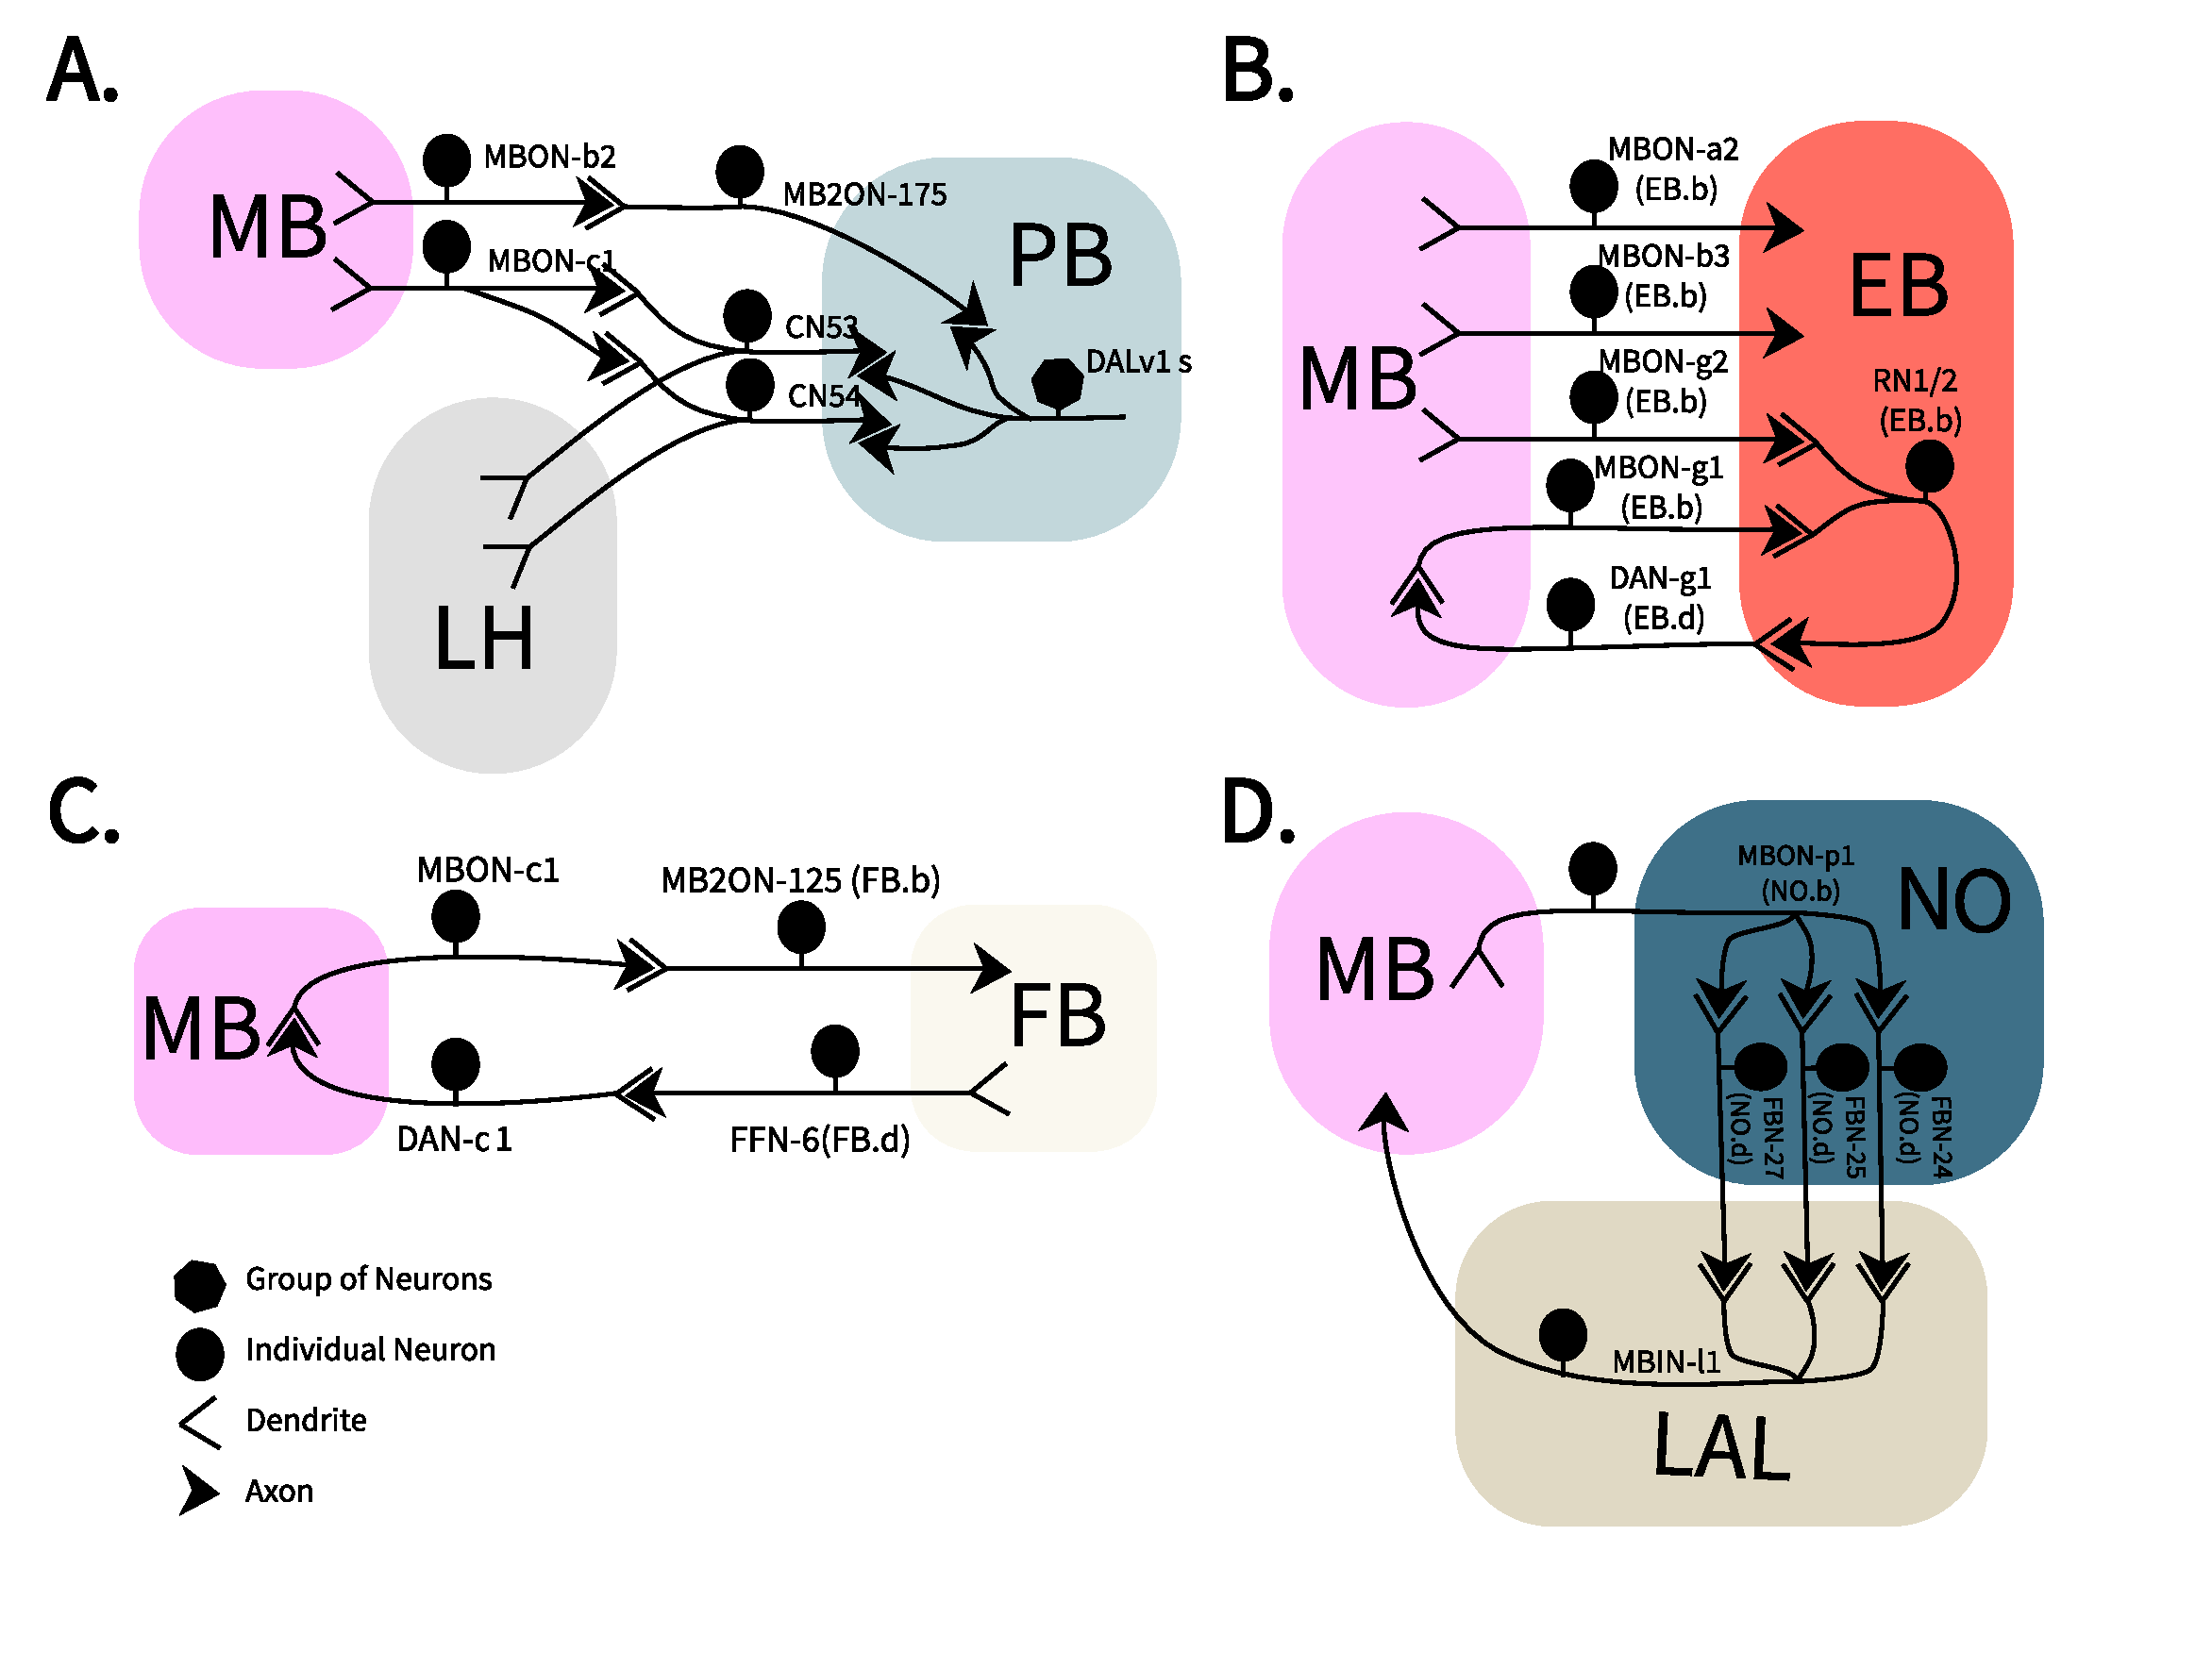
\includegraphics[width=17cm]{Figs/CX/MBtoCX.pdf}
        \caption[Mushroom Body Connections to the Larval CX]{Mushroom Body Connections to the Larval CX}
        \label{MBtoCX}
    \end{figure}

    \subsubsection{A loop between FB and the 'c' compartment of the MB}
    % MBON-c1 -> MB2ON-125 (FB.b) -> FFN-6 (FB.d) -> DAN-c1  
    We found that MBON-c1 synapses onto one FB.b neuron, MB2ON-125.
    Interestingly, DAN-c1 integrates inputs from an FB.d neuron, FFN-6, which in turn integrates inputs from a few neurons that are directly postsynaptic to MB2ON-125, defining a loop between the MB 'c' compartment and the FB.
    No other MBON supplies direct or two-hop inputs onto the FB.

    % EB to MB
    \subsubsection{Reciprocal connectivity between EB ring neurons and the 'g' compartment of the MB}
    % axo-axonic then axo-dendritic:
    % MBON-g1/g2 (EB.b) -> RN1/2 FBN-20 -> DAN-g1 (EB.d)
    Four MBONs (a2, b3, g1 and g2) are EB.b (i.e., deliver synapses to the EB; Fig. \ref{fig:mbtocx}). Interestingly, some of these MBONs are monosynaptically interrelated, namely MBON-g1 and -g2 (which promote approach) are GABAergic neurons that synapse onto MBON-a2 (which promote avoidance) \citep{eschbach2021circuits}.
    Furthermore, MBON-g1 and -g2 synapse axo-axonically onto an EB ring neuron, RN1/2 (also known as FBN-20; \citep{eschbach2021circuits}), a core GABAergic neuron of the EB, which in addition to synapting axo-axonically recyprocally onto EB wedge neurons also synapses onto an EB.d neuron, DAN-g1.
    Therefore, the output of the MB 'g' compartment (MBON-g1 and -g2) modulate, with GABA, the axon of an EB ring neuron (RN1/2), which in turn synapses onto the dendrites of the teaching neuron of the MB 'g' compartment (DAN-g1).
    This circuit configuration defines a close relationship between an associative learning compartment (MB 'g') and the EB.

    Assuming the larval ring neurons RN1/2 are also GABAergic, as they are in the adult \citep{hanesch1989neuronal}, the MB 'g' compartment is providing disinhibitory input onto the EB, by means of MBON-g1/g2 inhibiting its ring neurons.
    This disinhibition could be understood as a learning-based gating mechanism over EB wedge neurons, with features of input space expressed in the Kenyon cell population code, by coincident activity with DAN-g1, modulating the activity of the EB wedge neurons that the ring neurons also synapse onto.
    Taken together, this implies that, if the larval EB is functionally similar to that of the adult EB, there is a component of learning built-in into the internal representation of the direction of movement.

    \subsubsection{A loop between the NO and the MB vertical lobe via the LAL}
    % All are axo-dendritic synapses:
    % MBON-p1 (NO.b) -> FBN-24/25/27 (NO.d) -> MBIN-l1

    MBON-p1 is a multi-compartment MBON of the MB vertical lobe that is an NO.b, (i.e., it delivers output synapses to the NO).
    At the NO, MBON-p1 synapses onto several NO.d neurons, FBN-24, FBN-25, and FBN-27, which are MB feedback neurons \citep{eschbach2020recurrent} that all project to the LAL and synapse strongly onto MBIN-l1, a MB input neuron targeting multiple compartments of the vertical lobe.
    This circuit configuration defines a strong tight loop between the MB vertical lobe and the NO via the LAL.

    Note that the dendrites of MBIN-l1 are entirely contained within the LAL compartment.
    In addition, these three feedback neurons also synapse weakly onto DAN-d1.


    \subsubsection{The MB modulates inputs to the PB}
    % MBON-d1 -> MB2ON-63 (PB.b) -> multiple PB.d (some are NO.b like MB2ON-241)
    % CN-53, CN-54, MB2ON-175 all synapse onto DALv1 neurons

    % VISUAL input to the PB and the EB
    Multiple sensory modalities converge onto the horizontal fibers of the PB (DALv1 neurons) via MB convergence neurons (CN-53, CN-54) and a neuron postsynaptic to MBONs (MB2ON-175).
    These CNs were previously described as integrating the output of both the lateral horn (LH), which conveys innate pathways, and the mushroom body (MB), for associative memory \citep{eschbach2021circuits}.
    Synapses from CN-53, CN-54 and MB2ON-175 onto PB horizontal fiber neurons (DALv1) follow an intriguing pattern of synapting onto either the dendrite or the axon, but largely not both, with specific target choices among the 4 DALv1 neurons.
    In considering that 3 of the 4 DALv1 neurons (PB horizontal fibers) present an unusual bilateral axon that first deploys output synapses contralaterally and then ipsilaterally (Fig. \ref{fig:dalv1neurons}A), the observed pattern of selective axo-dendritic and axo-axonic connections has implications for the modulation of the output of the unusual axons of DALv1 neurons.


    In summary, from the perspective of the PB, we find the following circuit architecture: the multi-sensory convergence onto the PB horizontal fibers is directly modulated by the MB, precisely because the neurons that mediate the multi-sensory convergence are themselves CNs (i.e., integrate also MBON synapses in addition to LH inputs): the CN-53 and CN-54. %Both of these neurons are also Lateral Horn (LH) neurons.
    Note CN-54 is in addition a PB.d neuron, integrating inputs from PB horizontal fibers (DALv1 neurons).

    Upstream, among various MBONs, MBON-c1 is the most strongly connected to both CN-53 and CN-54, which also integrate inputs from MBON-b1 and MBON-b2. All three are MBONs of the MB peduncle; MBON-c1 has no known function, while MBON-b1 and MBON-b2 promote approach \citep{eschbach2021circuits}.

    Of note, the axon of MBON-c1 receives direct presumably inhibitory (GABAergic) inputs from MBON-g1, MBON-g2, and MBON-d1, with all three MBONs participating of circuit loops with other central complex neuropils.

    Additionally, neurons directly postsynaptic to MBONs, such as MB2ON-175, in turn directly synapse onto the horizontal fibers of the PB, either axo-axonically or axo-dendritically, in a pattern selective of specific DALv1 neurons.

    In summary, not only are navigational decisions such as whether to turn to stimuli or not proceeding not independently per sensory modality but integrated across modalities, as observed before in behavioral experiments \citep{gepner2015computations}, but also such integration is modulated by prior memories.

    %Vertical lobe is used by the NO and MB and LAL.
    %mb2on-c1 has no results(when it comes to aversion), but massively related to EB so it might 
    %mb2in-l1 according to eschback all the compartments of vertical love are for aversive behaviour.only mnbin that is not bilateral.  
    %m2on-p1 noduli itself gets input from(..) 
    % (extended data figure 6a - complete connectome of learning memory centre) 
    % ipsilateral control via these only mbons and mbins that are ipsilateral as opposed to bilateral. 


















\section{Dopaminergic neurons (DANs) of the larval central complex}
    
    \begin{figure}
        \centering
        \includegraphics[width=17cm]{Figs/CX/DANs.pdf}
        \caption{Confocal Images of Immunostained Dopaminergic neurons of the Larval Central Complex}
        \label{DANs}
    \end{figure}

Dopaminergic release outside the MB in the adult fly is known to trigger sleep via dorsal FB (dFB) neurons~\citep{pimentel2016sleep}, among other potential roles, depending upon the dopamine receptors expressed in the postsynaptic neurons and the circuits the neurons are part of.

The larval MB houses 7 pairs of DANs \citep{eichler2017complete}, with several more DANs scattered across the brain \citep{selcho2009thgal4}. By flp-out of the TH-GAL4 expression pattern that encompasses all DANs \citep{selcho2009thgal4} followed by immunohistochemistry, we isolated individual neurons from the TH-GAL4 expression patteern and compared their morphology with EM-reconstructed brain neurons \citep{winding2023connectome}. We identified with reasonable certainty the following 5 eDAN types (eDAN for \textit{external} DAN, i.e., not a MB DAN), comprising 6 neuron pairs.

\textbf{eDAN-1}: from the larval lineage DPMpm2, this neuron presents an ipsilateral dendrite in the posterior-dorsal brain, and a bilateral axon exactly overlapping with HF-PB dendrites. eDAN-1 integrates inputs from PB.d neurons like CN-54 (which mediates multi-sensory input integration and relays them to HF-PB, modulated by MB output; see above) but also from multiple sensory PNs such as for temperature (Suckerfish PN, Thermo PN 3 and Thermo PN 5), olfaction (mPN A3), and for unknown sensory modalities (Suckerfish PN 2, from unknown sensory MN-Sens-B2-ACp-21 and -22; \citep{miroschnikow2018convergence}), and also from PB.b neurons like MB2ON-63. The axon of eDAN-1 synapses onto multiple PB.d neurons (MB2ON-187, CN-15, CN-54, ADC1, FB-LAL1, and SP2-1) and weakly onto HF-PB neurons.

\textbf{eDAN-2}: from the larval lineage CM4-dm, this DAN presents a small, compact ipsilateral dendrite and a contralateral axon on the corresponding contralateral hemisphere right at the posterior end of the FB. eDAN-2 integrates inputs from FB neurons (strongly from FB.d.6, hs-FB.3, hs-FB.1, and weakly from many more). Its axon synapses onto MB2IN-195 (which is presynaptic to EB Wedge neurons), multiple FB neurons (hs-FB.3, hs-FB.1, FB.d.7 (FFN-6)), and weakly onto MB2IN-191 (the octopaminergic VUM of the CX).

\textbf{eDAN-3}: also known as MB2IN-139 \citep{eschbach2021circuits}, this neuron is from the larval lineage DPMpl12. Its dendrite is ipsilateral, sitting lateral to the FB but also extending into the LAL. The eDAN-3 axon targets a region dorsal to the LAL, housing the dendrites of  many EB.d neurons onto which it synapses, such as MB2IN-114, EB-DN1, MB2ON-17, EB wedge neurons (only W1), and many more neurons such as convergence neurons (CN-30, CN-37, CN-38, CN-41, CN-42, CN-43), MB2ON-256, and a peculiar FB.d.1 neuron (Bushy).

\textbf{eDAN-4}: this type consists of two nearly identical neurons that share most inputs but differ only slightly in their outputs, since their axons are juxtaposed but tiled medio-laterally. From the larval lineage DPMpl12, they present an ipsilateral dendrite in the posterior ventral brain and a contralateral axon in the posterior intermediate brain, beyond the limits of the FB proper. Both integrate inputs from numerous EB.d neurons like MB2IN-124, but only eDAN-4l (lateral axon) receives synapse from hs-FB.3. The axons of both eDAN-4 synapse onto some NO.d neurons like MB2ON-248 (whose dendrite has a domain in the NO and another outside where it meets the axon of both eDAN-4) and of other unidentified neurons (lasso-top 3, DALcm12-v descending), but only eDAN-4l synapses onto convergence neurons (CN-9, CN-26), and only eDAN-4m synapses onto hs-FB.5 and hs-FB.7.

\textbf{eDAN-5}: from the DPMpm1 larval lineage, this neuron's dendrite lays posterior to the LAL and projects its axon inside the lateral LAL. The dendrite integrates inputs from EB.d neurons, MB2IN-195, MB2ON-67, and sVUM2mx. The axon targets weakly but axo-dendritically an EB Ring neuron (RN1/2), and more strongly other neurons (MB2ON-67, MB2ON-78, MB2ON-68).

According to \citep{selcho2009thgal4} there are further non-MB DANs yet to be identified in the larval brain connectome. Note an effort was made to relate the eDANs we could identify to non-MB DAN names in \citep{selcho2009thgal4} but the resolution mismatch was too great to bridge, except for eDAN-1 which is most likely named "DM3" in \citep{selcho2009thgal4}.

%TODO: add eDAN-6 and eDAN-7



\section{Behavioral Assays - Loss of Function Analysis during light stimulation}
    \begin{figure}
        \centering
        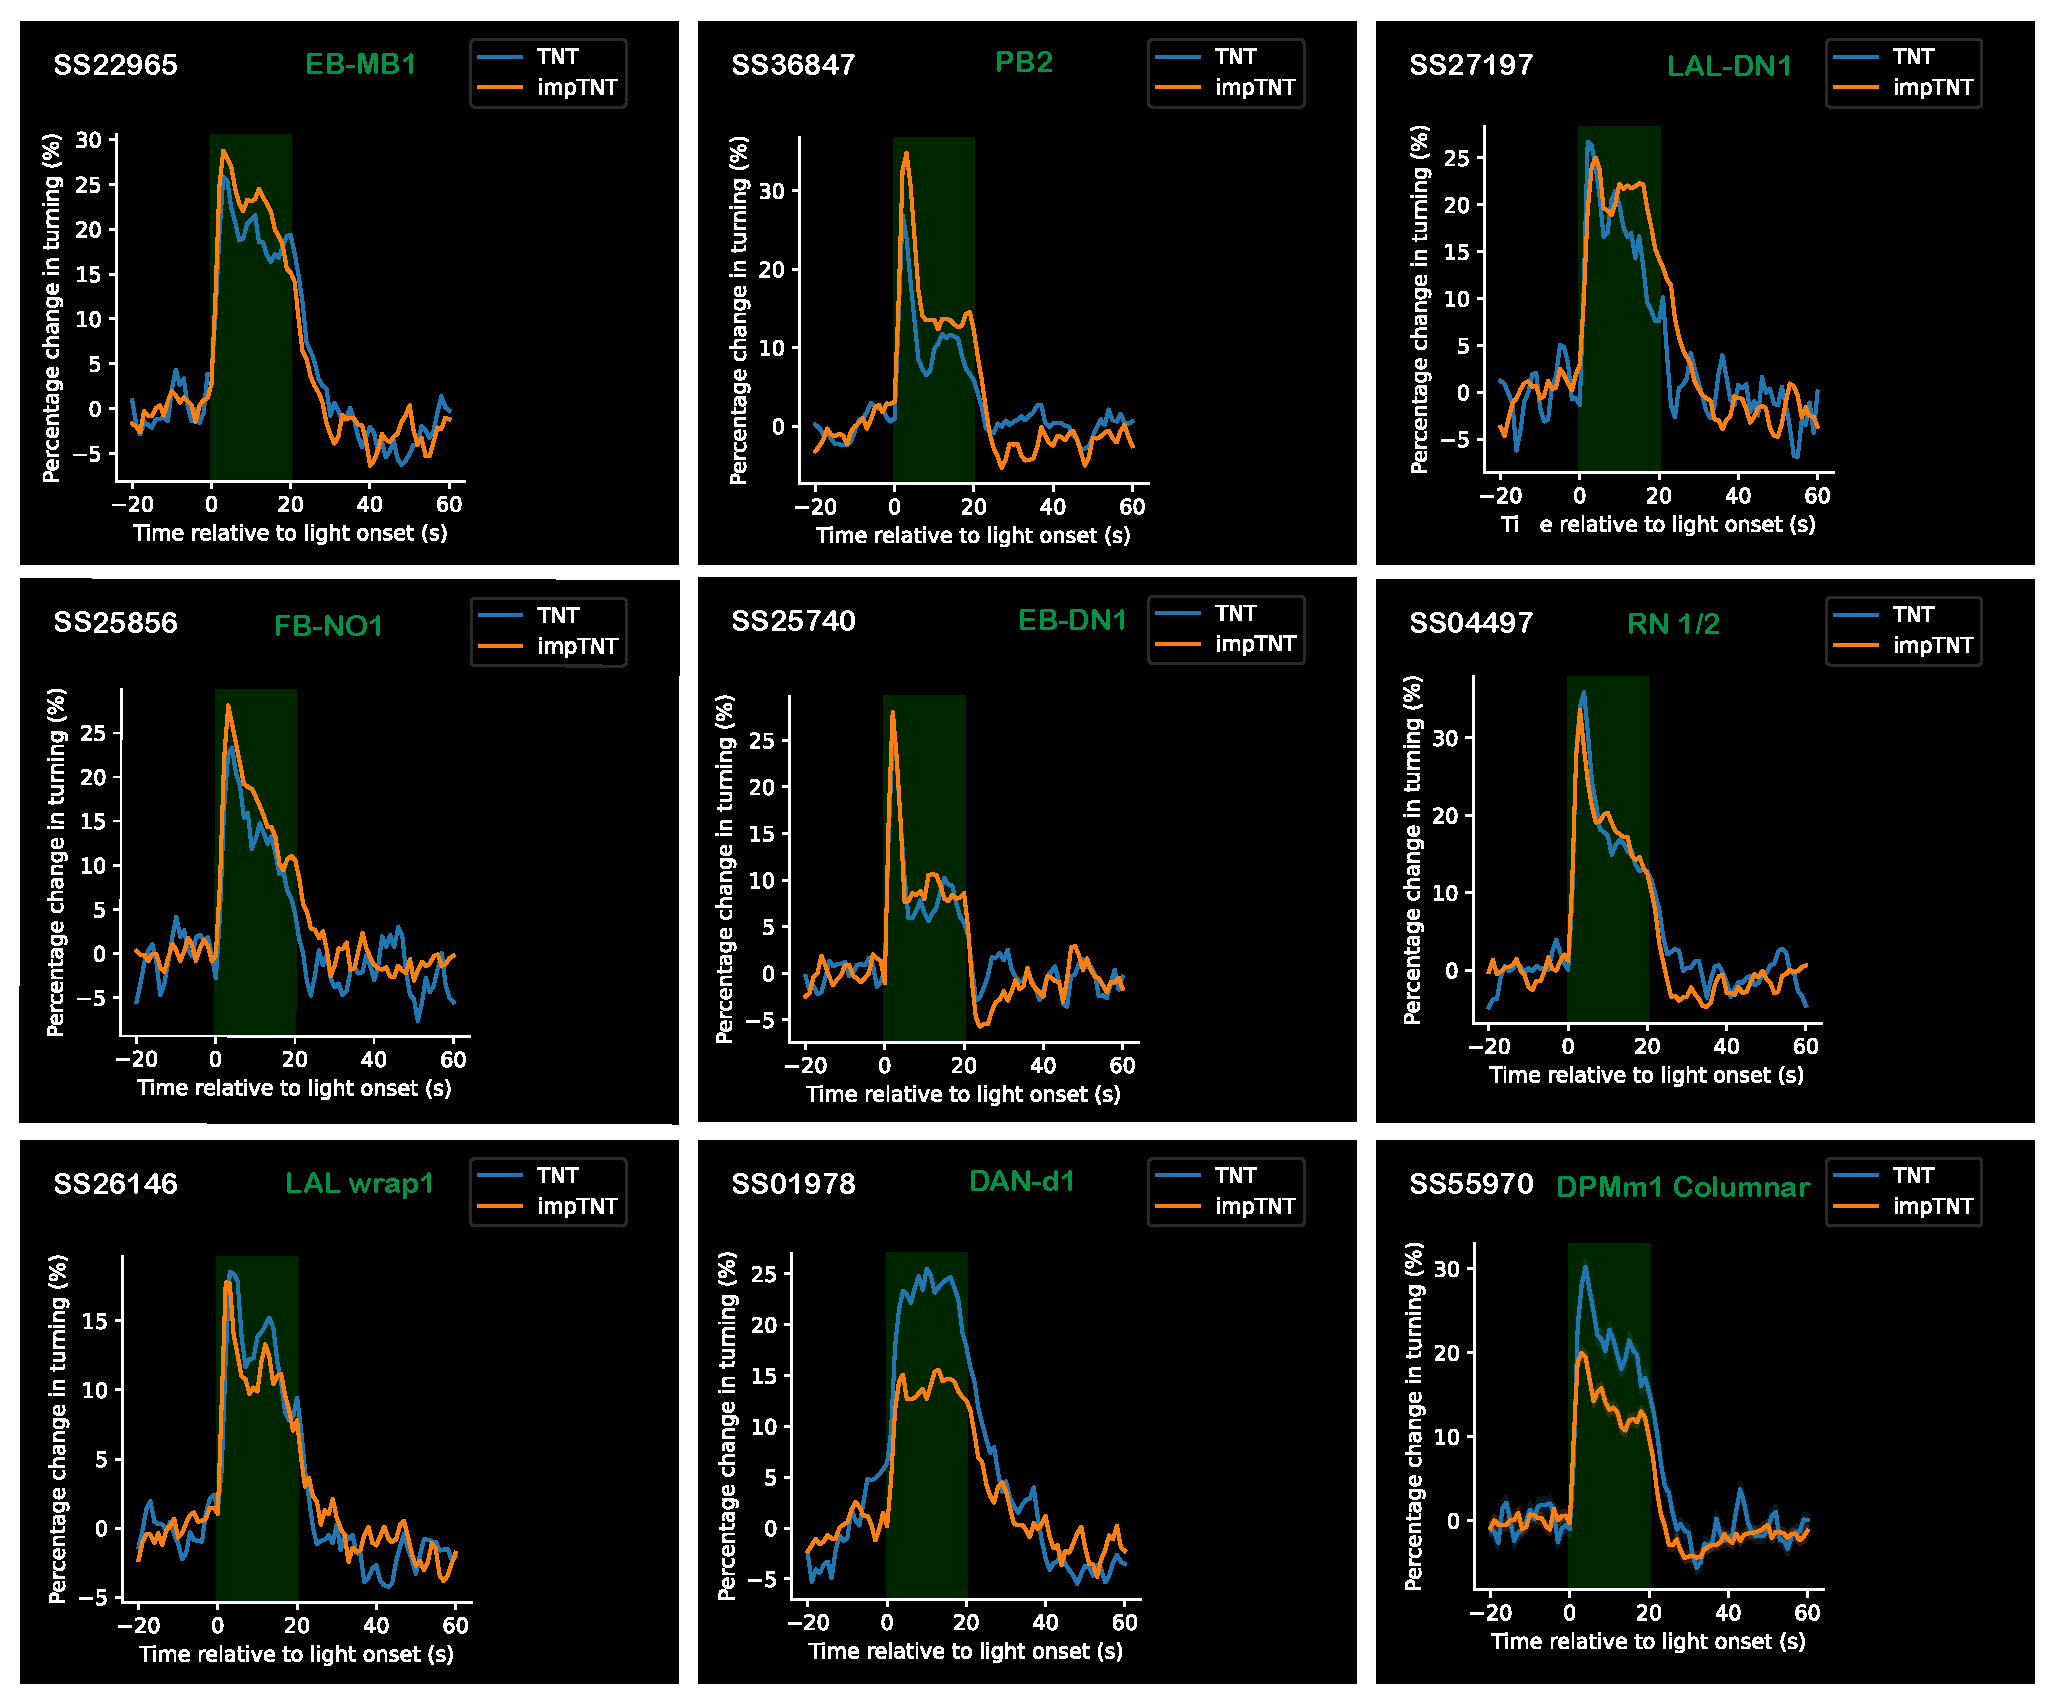
\includegraphics[width=12cm]{Figs/CX/BehaviourAssays.pdf}
        \caption[Loss of Function Analysis during Light Stimulation]{Loss of Function Analysis during Light Stimulation}
        \label{fig:label}
    \end{figure}


\section{Neural activity in response to blue light stimulation}
We were curious if the identified putative central comlpex would be responsive to light stimulation. 
We therefore monitored the activity across the entire larval brain in response to stimulation of Rh5 (blue senstitive) phtoreceptors. Photoreceptors (the Bolwig Organ) are located outside of the Central Nervous System(CNS) of Drosophila. We thus expressed  EGFP fluorescent tag in these neurons(Rh5s) to be to ensure they are present during dissection of the CNS and that they are preserved for mounting the sample in the glass capilary prior to Calcium Imaging. We created a final line that expresses green fluorescent RGECO (a calcium indicator of neural activity present cytosl) and red fluorescent IRFP (which brightens the cell nuclei very well and allows visualisation of cell position) and green fluorescent Rh5 photoreceptors. 


Upon blue light stimulation, we observed robust calcium transients in multiple regions of the larval brain.We expected the neuropil with the most visual input (Protocerebral Bridge) to be responsive. We segmented 

 This suggests that these structures are responsive to visual input mediated by Rh5 photoreceptors, supporting their functional role in sensory integration.



%To assess neural activity in response to blue light stimulation, we performed whole-brain calcium imaging using a transgenic line expressing green fluorescent RGECO (a cytosolic calcium indicator) and red fluorescent IRFP (a nuclear marker for cell position). EGFP was expressed in Rh5 photoreceptors (Bolwig Organ) to confirm their presence and integrity during CNS dissection and sample mounting.Upon blue light stimulation, we observed robust calcium transients in multiple regions of the larval brain, notably within the putative central complex neuropils, including the PB and EB. This suggests that these structures are responsive to visual input mediated by Rh5 photoreceptors, supporting their functional role in sensory integration.





    \begin{figure}
        \centering
        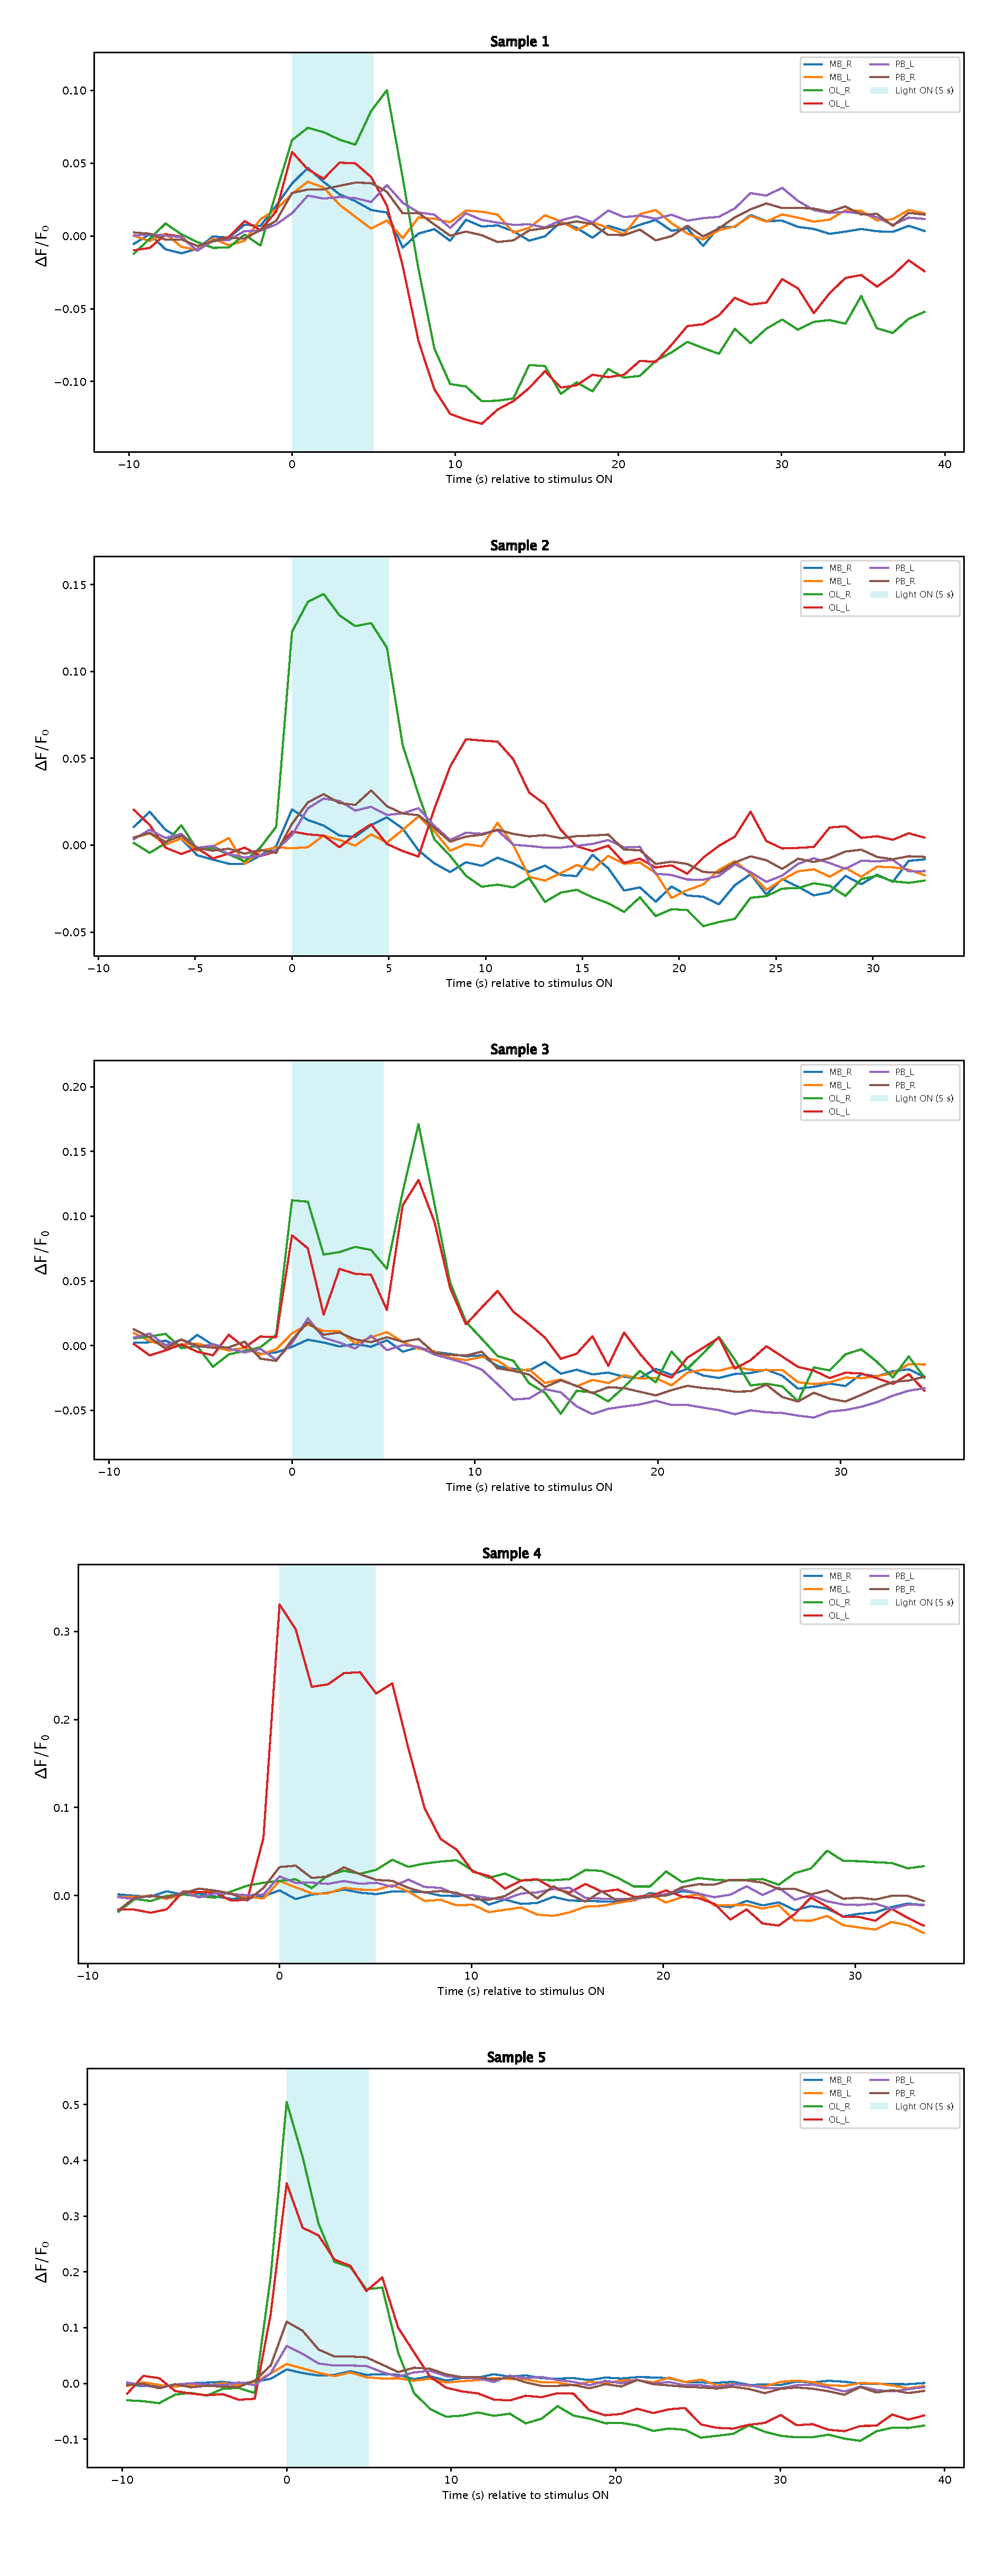
\includegraphics[width=10cm]{Figs/CX/RH5stimulation.pdf}
        \caption[Neural Activity of the Larval Brain in response to Photoreceptors Rh5 Stimulation]{Neural Activity of the Larval Brain in response to Photoreceptors Rh5 Stimulation}
        \label{RH5stimulation}
    \end{figure}


We observed Calcium transients. 


    


        
        

\section{Descending Neurons from CX}
        %catmaid annotation: 
            129 neurons descending to VNC
            93 neurons descending to SEZ
            216 total descending
            layer 1 annotated as: 'cx descending l1' (56 neurons) 25.6\%
            569 second order descending
            layer 2 annotated as: 'cx descending l2' (71 neurons of 569) 12.4\%



%\section{Visual input into the Larval Central Complex}%- 4 graphs showing connectivity between